\item Se realiza el siguiente experimento aleatorio: se lanza una moneda y un dado.
    \begin{enumerate}
        \item Definir un espacio muestral.\e\\
            La moneda puede resultar en cara o ceca, mientras que el dado en un natural menor o igual a 6.
            \begin{center}
                $X=$ cara\\
                $Y=$ ceca\\
            \end{center}
            Por lo tanto, el espacio muestral resulta ser\[\Omega=\{X1,X2,X3,X4,X5,X6,Y1,Y2,Y3,Y4,Y5,Y6\}\]
        \item Expresar explícitamente los siguientes sucesos:\\
            $A=$ "se obtiene un par y una cara".
            \[A=\{X2,X4,X6\}\]
            $B=$ "se obtiene un número primo".
            \[B=\{X2,X3,X5,Y2,Y3,Y5\}\]
            $C=$ "se obtiene un número impar y una ceca".
            \[C=\{Y1,Y3,Y5\}\]
        \item Encontrar expresiones para los siguientes eventos:
            \begin{enumerate}
                \item Sólamente ocurre $B$.\e\\
                    "Se obtiene un número primo"\e
                \item Ocurren tanto $A$ como $B$ pero no ocurre $C$.\e\\
                    "Se obtiene cara y un dos"\e
                \item Por lo menos dos ocurren.\e\\
                    Para ayudar a visualizar los eventos involucrados se realiza un diagrama de Venn
                    \begin{center}
                        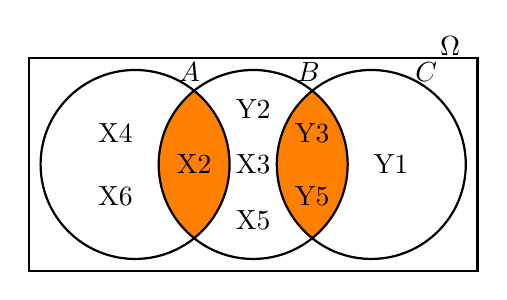
\begin{tikzpicture}
                            [thick,
                            set/.style = {circle,
                                        minimum size = 2cm}]
                            \begin{scope}
                                \clip (1.5,0) circle (1.2);
                                \clip (0,0) circle (1.2);
                                \fill[orange] (-1.35,-1.35) rectangle (4.35,1.35);
                            \end{scope}
                            \begin{scope}
                                \clip (1.5,0) circle (1.2);
                                \clip (3,0) circle (1.2);
                                \fill[orange] (-1.35,-1.35) rectangle (4.35,1.35);
                            \end{scope}
                            \draw [draw=black] (-1.35,-1.35) rectangle (4.35,1.35);
                            % Conjunto Metro
                            \node[set,label={65:$A$}] (A) at (0,0) {};
                            % Conjunto autobús
                            \node[set,label={65:$B$}] (B) at (1.5,0) {};
                            % Conjunto coche
                            \node[set,label={65:$C$}] (C) at (3,0) {};
                            \draw (0,0) circle(1.2cm);
                            \draw (1.5,0) circle(1.2cm);
                            \draw (3,0) circle(1.2cm);
                            \node at (-0.25,0.4) {X4};
                            \node at (-0.25,-0.4) {X6};
                            \node at (0.75,0) {X2};
                            \node at (1.5,0.7) {Y2};
                            \node at (1.5,0) {X3};
                            \node at (1.5,-0.7) {X5};
                            \node at (2.25,0.4) {Y3};
                            \node at (2.25,-0.4) {Y5};
                            \node at (3.25,0) {Y1};
                            \node at (4,1.5) {$\Omega$};
                        \end{tikzpicture}
                    \end{center}
                    En donde el área naranja es el evento de interés. Puedo expresar al evento como: "cara con 2 o ceca con impares mayores o iguales a 3".
                \item Ocurre uno y no más.
                    \begin{center}
                        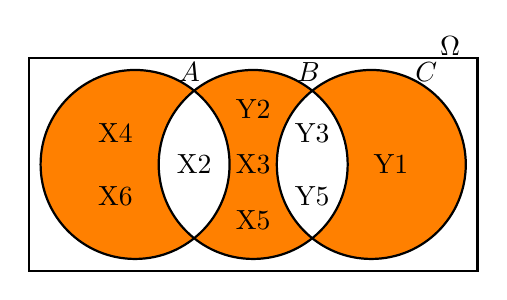
\begin{tikzpicture}
                            [thick,
                            set/.style = {circle,
                                        minimum size = 2cm}]
                            \fill[orange] (0,0) circle (1.2);
                            \fill[orange] (1.5,0) circle (1.2);
                            \fill[orange] (3,0) circle (1.2);
                            \begin{scope}
                                \clip (1.5,0) circle (1.2);
                                \clip (0,0) circle (1.2);
                                \fill[white] (-1.35,-1.35) rectangle (4.35,1.35);
                            \end{scope}
                            \begin{scope}
                                \clip (1.5,0) circle (1.2);
                                \clip (3,0) circle (1.2);
                                \fill[white] (-1.35,-1.35) rectangle (4.35,1.35);
                            \end{scope}
                            \draw [draw=black] (-1.35,-1.35) rectangle (4.35,1.35);
                            \node[set,label={65:$A$}] (A) at (0,0) {};
                            \node[set,label={65:$B$}] (B) at (1.5,0) {};
                            \node[set,label={65:$C$}] (C) at (3,0) {};
                            \draw (0,0) circle(1.2cm);
                            \draw (1.5,0) circle(1.2cm);
                            \draw (3,0) circle(1.2cm);
                            \node at (-0.25,0.4) {X4};
                            \node at (-0.25,-0.4) {X6};
                            \node at (0.75,0) {X2};
                            \node at (1.5,0.7) {Y2};
                            \node at (1.5,0) {X3};
                            \node at (1.5,-0.7) {X5};
                            \node at (2.25,0.4) {Y3};
                            \node at (2.25,-0.4) {Y5};
                            \node at (3.25,0) {Y1};
                            \node at (4,1.5) {$\Omega$};
                        \end{tikzpicture}
                    \end{center}
                    "Cara con número mayor a 2 o ceca con número menor a 3"
                \item No ocurren más de dos.
                \begin{center}
                    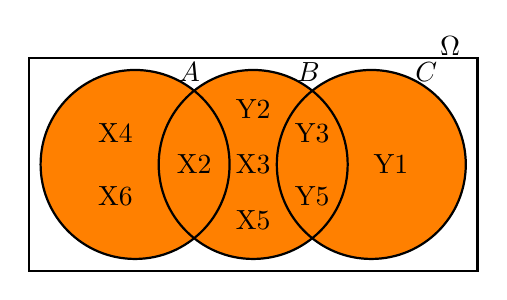
\begin{tikzpicture}
                        [thick,
                        set/.style = {circle,
                                    minimum size = 2cm}]
                        \fill[orange] (0,0) circle (1.2);
                        \fill[orange] (1.5,0) circle (1.2);
                        \fill[orange] (3,0) circle (1.2);
                        \draw [draw=black] (-1.35,-1.35) rectangle (4.35,1.35);
                        \node[set,label={65:$A$}] (A) at (0,0) {};
                        \node[set,label={65:$B$}] (B) at (1.5,0) {};
                        \node[set,label={65:$C$}] (C) at (3,0) {};
                        \draw (0,0) circle(1.2cm);
                        \draw (1.5,0) circle(1.2cm);
                        \draw (3,0) circle(1.2cm);
                        \node at (-0.25,0.4) {X4};
                        \node at (-0.25,-0.4) {X6};
                        \node at (0.75,0) {X2};
                        \node at (1.5,0.7) {Y2};
                        \node at (1.5,0) {X3};
                        \node at (1.5,-0.7) {X5};
                        \node at (2.25,0.4) {Y3};
                        \node at (2.25,-0.4) {Y5};
                        \node at (3.25,0) {Y1};
                        \node at (4,1.5) {$\Omega$};
                    \end{tikzpicture}
                \end{center}
                Como no hay intersección de los tres eventos, este evento es la unión de $A,B$ y $C$.
            \end{enumerate}
    \end{enumerate}